% ------------------------------------------------------------------------------
% TYPO3 CMS 6.2 LTS - What's New - Chapter "In-Depth Changes" (German Version)
%
% @author	Michael Schams <schams.net>
% @license	Creative Commons BY-NC-SA 3.0
% @link		http://typo3.org/download/release-notes/whats-new/
% @language	German
% ------------------------------------------------------------------------------
% Chapter: In-Depth Changes
% ------------------------------------------------------------------------------

\section{Änderungen im System}
\begin{frame}[fragile]
	\frametitle{Änderungen im System}

	\begin{center}\huge{Kapitel 6:}\end{center}
	\begin{center}\huge{\color{typo3darkgrey}\textbf{Änderungen im System}}\end{center}

\end{frame}

% ------------------------------------------------------------------------------
% normalize.css
% ------------------------------------------------------------------------------
% http://forge.typo3.org/issues/47920

\begin{frame}[fragile]
	\frametitle{Änderungen im System}
	\framesubtitle{Normalize.css}

	\begin{itemize}
		\item Das Backend nutzt nun \texttt{normalize.css}, dass dafür sorgt, dass Browser Elemente einheitlich unter Zuhilfenahme von modernen Webstandards dargestellt werden
		\item HTML5-ready und eine Alternative zu traditionellen CSS Reset Lösungen
		\item Ziele von \texttt{normalize.css} sind:

			\begin{itemize}
				\item Beibehaltung sinnvoller Voreinstellungen, anstatt diese nur zu überschreiben
				\item Normalisierung von Styles für diverse HTML Elemente 
				\item Behebung von Bugs und übliche Browser-Inkonsistenzen
				\item Usability-Steigerung durch raffinierte Verbesserungen
				\item Gute Dokumentation und Inline-Comments
			\end{itemize}

	\end{itemize}

\end{frame}

% ------------------------------------------------------------------------------
% displayCond options BIT and !BIT
% ------------------------------------------------------------------------------
% http://forge.typo3.org/issues/45514

\begin{frame}[fragile]
	\frametitle{Änderungen im System}
	\framesubtitle{TCA: displayCond Options BIT und !BIT}

	\lstset{
		basicstyle=\tiny\ttfamily
	}

	\begin{itemize}
		\item TCA \texttt{displayCond} bitweise gegen Multi-Value-Felder testen\newline
			\texttt{BIT}: Bit ist gesetzt, \texttt{!BIT}: Bit ist \underline{nicht} gesetzt
	\end{itemize}

	\begin{columns}[T]

		\begin{column}{.5\textwidth}

			\advance\leftskip+1cm
			\smaller
				Angenommen sei\newline
				folgendes TCA:
			\normalsize

			\lstset{xleftmargin=1cm}

			\begin{lstlisting}
				'content' => array(
				  'label' => '...',
				  'config' => array(
				    'type' => 'check',
				    'items' => array(
				      array('Content A', ''),
				      array('Content B', ''),
				      array('Content C', ''),
				    ),
				  )
				),
			\end{lstlisting}

		\end{column}
		\begin{column}{.5\textwidth}

			\smaller
				Anwendungs-\newline
				beispiele:
			\normalsize

			\begin{lstlisting}
				'content_a' => array(
				  'label' => '...',
				  'displayCond' => 'FIELD:content:BIT:1',
				  'config' => array(
				    'type' => 'text',
				  )
				),

				'content_b' => array(
				  'label' => '...',
				  'displayCond' => 'FIELD:content:!BIT:2',
				  'config' => array(
				    'type' => 'text',
				  )
				),
			\end{lstlisting}
		\end{column}

	\end{columns}

\end{frame}

% ------------------------------------------------------------------------------
% Automatic language updates for extensions
% ------------------------------------------------------------------------------
% http://forge.typo3.org/issues/43703

\begin{frame}[fragile]
	\frametitle{Änderungen im System}
	\framesubtitle{Automatisches Update für Sprachen}

	\begin{itemize}
		\item Ein Extbase Command Controller ermöglicht das automatische Update von Sprachen für Extensions:

			\begin{lstlisting}
				$GLOBALS['TYPO3_CONF_VARS']['SC_OPTIONS']['extbase']
				  ['commandControllers'][] =
				  'TYPO3\\CMS\\Lang\\Command\\LanguageCommandController';
			\end{lstlisting}

		\item Ein möglicher Aufruf wäre:

			\lstinline!typo3/cli_dispatch.phpsh extbase language:update de,en,fr!

		\item Eine komma-separierte Liste von Locales (e.g. \texttt{de,en,fr}) aktualisiert lediglich diese Sprachen
		\item Ohne dieses Argument werden alle Sprachen aktualisiert, die im Modul "Sprache" ausgewählt sind

	\end{itemize}

\end{frame}

% ------------------------------------------------------------------------------
% Migrate system extension manuals to reStructuredText
% ------------------------------------------------------------------------------
% http://forge.typo3.org/issues/50052

\begin{frame}[fragile]
	\frametitle{Änderungen im System}
	\framesubtitle{System Extension: ReST Manuals}

	\begin{itemize}
		\item Manuals sämtlicher System Extensions wurde zu reStructuredText migriert
		\item OpenOffice Manuals werden nicht länger benötigt und wurde entfernt
		\item ReST ist ein leicht zu lesendes, "what-you-see-is-what-you-get", Text-basiertes Format
		\item ReST Dateien von System Extensions liegen unter:\newline
			\texttt{typo3/sysext/<extensionkey>/Documentation/*}

		\item Weitere Information unter:\newline
			\url{http://de.wikipedia.org/wiki/ReStructuredText}\newline
			\url{http://wiki.typo3.org/ReST}

	\end{itemize}

\end{frame}

% ------------------------------------------------------------------------------
% Support custom translation servers for extensions
% ------------------------------------------------------------------------------
% http://forge.typo3.org/issues/50052

\begin{frame}[fragile]
	\frametitle{Änderungen im System}
	\framesubtitle{Eigene Übersetzungsserver für Extensions}

	\begin{itemize}
		\item Durch XLIFF und einem neuen Signal/Slot können nun eigene Übersetzungsserver für Extensions eingesetzt werden\newline
			\small(nächste Slide zeigt ein Beispiel)\normalsize
		\item Eine mögliche Lösung für einen Übersetzungsserver: \textbf{Pootle}

			\begin{itemize}
				\item Online Translation Management Tool
				\item geschrieben in Python/Django
				\item original entwickelt und veröffentlicht von \url{translate.org.za}
				\item freigegeben unter GNU GPL
			\end{itemize}

	\end{itemize}

\end{frame}

% ------------------------------------------------------------------------------
% Support custom translation servers for extensions
% ------------------------------------------------------------------------------
% http://forge.typo3.org/issues/50052

\begin{frame}[fragile]
	\frametitle{Änderungen im System}
	\framesubtitle{Eigene Übersetzungsserver für Extensions}

	Beispiel: \texttt{EXT:myextension/localconf.php}

	\lstset{
		basicstyle=\tiny\ttfamily
	}

	\begin{lstlisting}
		/**
		 * @var \TYPO3\CMS\Extbase\SignalSlot\Dispatcher $signalSlotDispatcher
		 */
		$signalSlotDispatcher =
		  \TYPO3\CMS\Core\Utility\GeneralUtility::makeInstance(
		    'TYPO3\\CMS\\Extbase\\SignalSlot\\Dispatcher');

		$signalSlotDispatcher->connect(
		  'TYPO3\\CMS\\Lang\\Service\\UpdateTranslationService',
		  'postProcessMirrorUrl',
		  'Company\\Extension\Slots\\CustomMirror',
		  'postProcessMirrorUrl'
		);
	\end{lstlisting}

\end{frame}

% ------------------------------------------------------------------------------
% Support custom translation servers for extensions
% ------------------------------------------------------------------------------
% http://forge.typo3.org/issues/50052

\begin{frame}[fragile]
	\frametitle{Änderungen im System}
	\framesubtitle{Eigene Übersetzungsserver für Extensions}

	Beispiel: \texttt{EXT:myextension/Classes/Slots/CustomMirror.php}

	\lstset{
		basicstyle=\tiny\ttfamily
	}

	\begin{lstlisting}
		<?php
		namespace Company\Extensions\Slots;
		class CustomMirror {

		  /**
		   * @var string
		   */
		  protected static $extKey = 'myextension';

		  public function postProcessMirrorUrl($extensionKey, &$mirrorUrl) {
		    if ($extensionKey === self::$extKey) {
		      $mirrorUrl = 'http://example.com/typo3-packages/';
		    }
		  }

		}
	\end{lstlisting}

\end{frame}

% ------------------------------------------------------------------------------
% Support custom translation servers for extensions
% ------------------------------------------------------------------------------
% http://forge.typo3.org/issues/50052

\begin{frame}[fragile]
	\frametitle{Änderungen im System}
	\framesubtitle{Eigene Übersetzungsserver für Extensions}

	Vorausgesetzte Datei/Verzeichnis-Struktur auf dem Server:

	\begin{lstlisting}
		http://example.com/typo3-packages/
		 `-- <first-letter-of-extension-key>
		     `-- <second-letter-of-extension-key>
		         `-- <extension-key>-l10n
		             |-- <extension-key>-l10n-de.zip
		             |-- <extension-key>-l10n-fr.zip
		             |-- <extension-key>-l10n-it.zip
		             `-- <extension-key>-l10n.xml
	\end{lstlisting}

	Zum Beispiel:

	\begin{lstlisting}
		http://example.com/typo3-packages/m/y/myextension-l10n/myextension-l10n.xml
	\end{lstlisting}

\end{frame}

% ------------------------------------------------------------------------------
% Support custom translation servers for extensions
% ------------------------------------------------------------------------------
% http://forge.typo3.org/issues/50052

\begin{frame}[fragile]
	\frametitle{Änderungen im System}
	\framesubtitle{Eigene Übersetzungsserver für Extensions}

	Beispiel: \texttt{<extension-key>-l10n.xml}

	\lstset{
		basicstyle=\tiny\ttfamily
	}

	\begin{lstlisting}
		<?xml version="1.0" standalone="yes" ?>
		  <TERlanguagePackIndex>
		    <meta>
		      <timestamp>1374841386</timestamp>
		      <date>2013-07-26 14:23:06</date>
		    </meta>
		    <languagePackIndex>
		    <languagepack language="de">
		      <md5>1cc7046c3b624ba1fb1ef565343b84a1</md5>
		    </languagepack>
		    <languagepack language="fr">
		     <md5>f00f73ae5c43cb68392e6c508b65de7a</md5>
		    </languagepack>
		    <languagepack language="it">
		     <md5>cd59530ce1ee0a38e6309544be6bcb3d</md5>
		    </languagepack>
		  </languagePackIndex>
		</TERlanguagePackIndex>
	\end{lstlisting}

\end{frame}

% ------------------------------------------------------------------------------
% Automatic import of t3d files for extensions
% ------------------------------------------------------------------------------
% http://forge.typo3.org/issues/51437

\begin{frame}[fragile]
	\frametitle{Änderungen im System}
	\framesubtitle{Automatisierter t3d Import}

	\begin{itemize}
		\item Extensions können während ihrer Installation nun automatisch\newline
			\textbf{t3d Packages} importieren
		\item t3d Packages beinhalten zum Beispiel Daten, Relationen, Dateien, usw.
		\item Die t3d Datei muss \texttt{data.t3d} lauten und sich in folgendem Verzeichnis befinden:
			\texttt{EXT:myextension/Initialisation/}
		\item Der Import geschieht nur \underline{einmalig}, selbst wenn die Extension später erneut installiert werden sollte
	\end{itemize}

\end{frame}

% ------------------------------------------------------------------------------
% Automatic import of files for extensions
% ------------------------------------------------------------------------------
% http://forge.typo3.org/issues/51446

\begin{frame}[fragile]
	\frametitle{Änderungen im System}
	\framesubtitle{Automatisierter Datei Import}

	\begin{itemize}
		\item Extensions können während ihrer Installation nun automatisch\newline
			\textbf{Dateien} importieren
		\item Dateien werden bereit gestellt unter:\newline
			\texttt{EXT:myextension/Initialisation/Files/...}
		\item Dateien werden während der Extension-Installation kopiert nach:\newline
			\texttt{fileadmin/<extensionkey>/}
		\item Der Import geschieht nur \underline{einmalig}, selbst wenn die Extension später erneut installiert werden sollte
	\end{itemize}

\end{frame}

% ------------------------------------------------------------------------------
% Use an extension as repository
% ------------------------------------------------------------------------------
% http://forge.typo3.org/issues/51835

\begin{frame}[fragile]
	\frametitle{Änderungen im System}
	\framesubtitle{Extensions als Repositories nutzen}

	\begin{itemize}
		\item Manchmal hängen Extensions von Extensions ab, die verändert und/oder angepasst wurden,
			oder von Extensions, die nicht im offiziellen TYPO3 Extension Repository (TER) veröffentlicht wurden
		\item Um diese Abhängigkeiten aufzulösen, können Extensions nun andere Extensions enthalten:\newline
			\texttt{EXT:myextension/Initialisation/Extensions/...}
		\item Während der Installation werden diese kopiert nach:\newline
			\texttt{typo3conf/ext/}
		\item Anschließend werden weitere Abhängigkeiten der Extension aufgelöst
	\end{itemize}

\end{frame}

% ------------------------------------------------------------------------------
% CLI command to install/uninstall extensions
% ------------------------------------------------------------------------------
% http://forge.typo3.org/issues/51629

\begin{frame}[fragile]
	\frametitle{Änderungen im System}
	\framesubtitle{(De-)Installation von Extensions über CLI}

	\begin{itemize}
		\item Extensions können nun via Command Line Interface (CLI), also über die Kommandozeile, installiert und de-installiert werden
		\item Beispiele:
			\lstinline!typo3/cli_dispatch.phpsh extbase extension:install <extensionkey>!
			\lstinline!typo3/cli_dispatch.phpsh extbase extension:uninstall <extensionkey>!

		\item Anmerkung: Backend-Benutzer \textbf{\_cli\_lowlevel} muss hierfür existieren!
	\end{itemize}

\end{frame}

% ------------------------------------------------------------------------------
% Enable/disable cascading deletion of child elements
% ------------------------------------------------------------------------------
% http://forge.typo3.org/issues/50391

\begin{frame}[fragile]
	\frametitle{Änderungen im System}
	\framesubtitle{TCA: Kaskadierendes Löschen von Datensätzen}

	\lstset{
		basicstyle=\tiny\ttfamily
	}

	\begin{itemize}
		\item Im TCA gibt es nun eine Einstellung, die es erlaubt, das kaskadierende Löschen von Kind-Datensätzen
ein- bzw. auszuschalten
		\item Dafür muss die Relation vom Typ "\textbf{inline}" sein
		\item Standardwert ist \texttt{TRUE}\newline
			\small(d.h. beim Löschen eines Datensatzes werden die Kind-Datensätze automatisch mitgelöscht)\normalsize
		\item Beispiel (Deaktivierung der Löschung von Kind-Datensätzen):

			\begin{lstlisting}
				...
				'type' => 'inline',
				'foreign_table' => ...,
				  'behaviour' => array(
				    'enableCascadingDelete' => 0
				  )
				  ...
				)
				...
			\end{lstlisting}

	\end{itemize}

\end{frame}

% ------------------------------------------------------------------------------
% Multiple category fields per table
% ------------------------------------------------------------------------------
% http://forge.typo3.org/issues/51921

\begin{frame}[fragile]
	\frametitle{Änderungen im System}
	\framesubtitle{Mehrere Kategorien pro Tabelle}

	\begin{itemize}
		\item Bisher konnte nur \underline{ein} \texttt{makeCategorizable()}-Aufruf per Tabelle ausgeführt werden\newline
			\small(weitere Aufrufe überschrieben die vorhergehenden)\normalsize
		\item Seit TYPO3 CMS 6.2 können beliebig viele solcher Felder existieren
		\item Beispiel:

			\begin{lstlisting}
				\TYPO3\CMS\Core\Utility\ExtensionManagementUtility::makeCategorizable(
				  $extensionKey,
				  $tableName,
				  $fieldName = 'categories',
				  $options = array(
				  	'label' => 'my category'
				  )
				);
			\end{lstlisting}

		\item Mit \texttt{\$options} kann ein eigenes Label für das Feld eingebracht werden

	\end{itemize}

\end{frame}

% ------------------------------------------------------------------------------
% Backend layout data providers
% ------------------------------------------------------------------------------
% http://forge.typo3.org/issues/37208

\begin{frame}[fragile]
	\frametitle{Änderungen im System}
	\framesubtitle{Data Provider für Backend Layouts}

	\begin{itemize}
		\item In TYPO3 vor Version 6.2 werden Backend Layouts ausschließlich in der Datenbank gespeichert
		\item Seit TYPO3 ab Version 6.2 können sogenannte \emph{Data Provider} definiert werden\newline
			\small(Extensions können somit ihre eigenen Backend Layout Definitionen liefern)\normalsize

		\item Data Provider müssen das folgende Interface implementieren:\newline
			\smaller\texttt{
				TYPO3\textbackslash\textbackslash
				CMS\textbackslash\textbackslash
				Backend\textbackslash\textbackslash
				View\textbackslash\textbackslash
				BackendLayout\textbackslash\textbackslash
				DataProviderInterface}\normalsize

		\item und werden wie folgt registriert:

			\begin{lstlisting}
				$GLOBALS['TYPO3_CONF_VARS']['SC_OPTIONS']
				  ['BackendLayoutDataProvider'][$_EXTKEY] = 'Classname';
			\end{lstlisting}


	\end{itemize}

\end{frame}

% ------------------------------------------------------------------------------
% Backend layout data providers
% ------------------------------------------------------------------------------
% http://forge.typo3.org/issues/37208

\begin{frame}[fragile]
	\frametitle{Änderungen im System}
	\framesubtitle{Backend Layout Data Providers}

	\begin{itemize}
		\item Zudem gibt es neue API-Befehle für das Backend Layout Handling, z.B.:

			\begin{lstlisting}
				'itemsProcFunc' => 'TYPO3\\CMS\\Backend\\View\\
				  BackendLayoutView->addBackendLayoutItems'
			\end{lstlisting}

			\begin{lstlisting}
				getBackendLayoutView()->getSelectedCombinedIdentifier($id);
				getBackendLayoutView()->getSelectedBackendLayout();
			\end{lstlisting}

		\item PageTSconfig Option, um Backend Layouts von der Zuweisung auszuschließen:

			\begin{lstlisting}
				options.backendLayout.exclude = default_1, my_extension__headerLayout
			\end{lstlisting}

	\end{itemize}

\end{frame}

% ------------------------------------------------------------------------------
% Filter for multiple value selector
% ------------------------------------------------------------------------------
% http://forge.typo3.org/issues/49739

\begin{frame}[fragile]
	\frametitle{Änderungen im System}
	\framesubtitle{Multiple Value Selector (1)}

	\begin{itemize}
		\item Ein Filter ermöglicht es, Einträge in einem Multi-Select Feld auszublenden, um die Suche deutlich zu vereinfachen
		\item Dafür muss das TCA entsprechend angepasst werden\newline
			\small(z.B. in der Datei \texttt{typo3conf/extTables.php}):\normalsize

			\lstset{
				basicstyle=\tiny\ttfamily
			}

			\begin{lstlisting}
				$GLOBALS['TCA']['fe_users']['columns']['usergroup']['config']
				  ['enableMultiSelectFilterTextfield'] = TRUE;

				$GLOBALS['TCA']['fe_users']['columns']['usergroup']['config']
				  ['multiSelectFilterItems'] = array(

				  array('',     'show all'),  // no filter
				  array('test', 'test'),      // first value: filter, second value: label

				  array(
				    'TYPO3',
				    'LLL:EXT:myext/Resources/Private/Language/locallang_db.xlf:tx_myext.label.typo3'
				  ),
				);
			\end{lstlisting}

	\end{itemize}

\end{frame}

% ------------------------------------------------------------------------------
% Filter for multiple value selector
% ------------------------------------------------------------------------------
% http://forge.typo3.org/issues/49739

\begin{frame}[fragile]
	\frametitle{Änderungen im System}
	\framesubtitle{Multiple Value Selector (2)}

	\begin{itemize}
		\item Zwei Optionen stehen zur Verfügung:

			\begin{itemize}
				\item Auswahl aus einer Dropdown Box mit vordefinierten Begriffen
				\item Textfeld zur Eingabe eines Such/Filter-Begriffes
			\end{itemize}

		\item Das Ergebnis könnte dann beispielsweise wie folgt aussehen:
	\end{itemize}

	\begin{figure}
		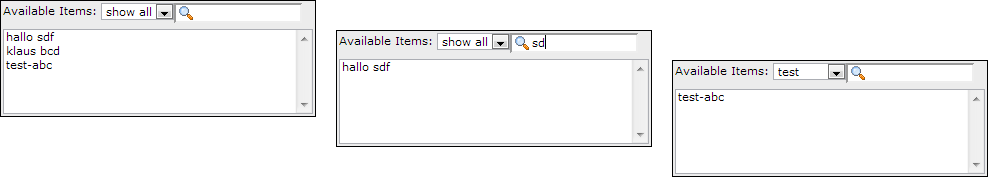
\includegraphics[width=1\linewidth]{Images/InDepthChanges/MultipleValueSelector.png}
	\end{figure}

\end{frame}

% ------------------------------------------------------------------------------
% Improved caching framework by introducing cache groups
% ------------------------------------------------------------------------------
% http://forge.typo3.org/issues/54991

\begin{frame}[fragile]
	\frametitle{Änderungen im System}
	\framesubtitle{Cache Gruppen (1)}

	\begin{itemize}
		\item Der TYPO3 Core nutzt nun zwei verschiedene Cache Gruppen:

			\begin{itemize}
				\item \textbf{System Caches}:
				class loading cache, configuration cache, l10n\_cache, extbase\_object, extbase\_reflection etc.
				\item \textbf{Frontend Caches}:
				cHash cache, page cache, page section cache
			\end{itemize}

		\item In TYPO3 vor 6.2 leerte \textit{clear all caches} \underline{sämtliche} Caches (nicht ideal)

		\item In TYPO3 ab 6.2 macht der Core Gebrauch von zwei Cache Gruppen:\newline
			"\textbf{pages}" für alle Seiten-relavanten Caches und "\textbf{system}", welches für Compile-Time und Konfigurations-Caches zuständig ist

	\end{itemize}

	\begin{figure}
		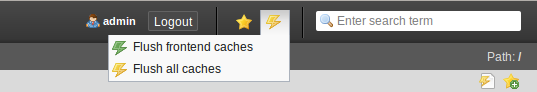
\includegraphics[width=0.5\linewidth]{Images/InDepthChanges/CacheGroups.png}
	\end{figure}

\end{frame}

% ------------------------------------------------------------------------------
% Improved caching framework by introducing cache groups
% ------------------------------------------------------------------------------
% http://forge.typo3.org/issues/54991

\begin{frame}[fragile]
	\frametitle{Änderungen im System}
	\framesubtitle{Cache Groups (2)}

	\lstset{
		basicstyle=\tiny\ttfamily
	}

	\begin{itemize}

		\item Entsprechende Konfigurationsoption:\newline
			\smaller(in den Dateien: \texttt{LocalConfiguration.php}/\texttt{DefaultConfiguration.php})\normalsize

			\begin{lstlisting}
			'cache_hash' => array(
			  'frontend' => 'TYPO3\CMS\Core\Cache\Frontend\VariableFrontend',
			  'backend' => 'TYPO3\CMS\Core\Cache\Backend\Typo3DatabaseBackend',
			  'options' => array(),
			  'groups' => array('pages', 'all')
			),
			\end{lstlisting}

		\item "\textit{Flush all caches}" leert nicht mehr System Caches\newline
			\small(nur "\textit{Clear Configuration Cache}" oder das Install Tool leert diese)\normalsize
		\item Neue userTSconfig Option ermöglicht es Nicht-Admins System Caches zu leeren:\newline
			\smaller\texttt{options.clearCache.system = 1}\normalsize

		\breakingchange

	\end{itemize}

\end{frame}

% ------------------------------------------------------------------------------
% TCA: limit number of ticked checkboxes
% ------------------------------------------------------------------------------
% http://forge.typo3.org/issues/55187
% http://forge.typo3.org/issues/55188 (documentation: TCA reference)

\begin{frame}[fragile]
	\frametitle{Änderungen im System}
	\framesubtitle{TCA: Anzahl Aktivierte Checkboxen}

	\lstset{
		basicstyle=\tiny\ttfamily
	}

	\begin{itemize}
		\item TCA erlaubt nun die Prüfung/Limitierung der Anzahl aktivierter Checkboxen

			\begin{itemize}
				\item \texttt{maximumRecordsChecked}:\newline
					Limitiert die maximale Anzahl Datensätze von der selben Tabelle
				\item \texttt{maximumRecordsCheckedInPid}:\newline
					Limitiert die maximale Anzahl Datensätze auf der selben PID (parent ID)
			\end{itemize}

		\item Wählt der Backend Benutzer weitere Checkboxen nach dem erreichen der maximal zulässigen Anzahl aus, so werden diese wieder deaktiviert

		\item Example:

			\begin{lstlisting}
				$tcaConfiguration = array(
				  'type' => 'check',
				  'eval' => 'maximumRecordsChecked',
				  'validation' => array(
				    'maximumRecordsChecked' => 5
				  )
				);
			\end{lstlisting}

	\end{itemize}

\end{frame}

% ------------------------------------------------------------------------------
% TCA: Introduce MM_oppositeUsage property
% ------------------------------------------------------------------------------
% http://forge.typo3.org/issues/56061
% http://forge.typo3.org/issues/56123 (documentation: TCA reference)

\begin{frame}[fragile]
	\frametitle{In-Depth Changes}
	\framesubtitle{TCA: \texttt{MM\_oppositeUsage} Eigenschaft}

	\lstset{
		basicstyle=\tiny\ttfamily
	}

	\begin{itemize}
		\item Wenn ein \texttt{sys\_category} Datensatz kopiert wird, wird eine neue MM-Referenz angelegt, allerdings
ohne den "fieldname" zu setzen
		\item Der Wert wird prinzipiell von der Gegenseite mittels \texttt{MM\_match\_fields} definiert, auf den man allerdings bislang nicht zugreifen konnte
		\item Um dieses Problem zu lösen, wurde die neue Eigenschaft \texttt{MM\_oppositeUsage} eingeführt:

			\begin{lstlisting}
				'config' => array(
				  'allowed' => '*',
				  'MM' => 'tx_myextension_first_second_mm',
				  'MM_oppositeUsage' => array(
				    'tt_content' => array('somefield'),
				    'tx_myextension_domain_model' => array('some_property'),
				  ),
				),
			\end{lstlisting}

	\end{itemize}

\end{frame}

% ------------------------------------------------------------------------------
% Miscellaneous
% ------------------------------------------------------------------------------
% http://forge.typo3.org/issues/49037 (Custom record list in element browser)
% http://forge.typo3.org/issues/36505 (Increase size of be_groups.subgroup field)
% http://forge.typo3.org/issues/49270 (Merge extensions TS/Template)

\begin{frame}[fragile]
	\frametitle{Änderungen im System}
	\framesubtitle{Diverses}

	\begin{itemize}

		\item \textbf{Eigene Record-List:}\newline
			\small
				Es ist nun möglich, eine eigene Record-List im Element-Browser zu verwenden und die Standard Record-List damit zu überschreiben.
			\normalsize

		\item \textbf{Mehr Untergruppen:}\newline
			\small
				Das Attribute \texttt{subgroup} in der Datenbank-Tabelle \texttt{be\_groups} wurde von \texttt{varchar(250)} zu \texttt{text} geändert, was die mögliche Anzahl von Untergruppen für Backend Benutzer deutlich steigert.
			\normalsize

		\item \textbf{Zusammengeführte TS/Template Extensions:}\newline
			\small
				Technisch gesehen war "WEB > Template" bisher auf mehrere Extensions verteilt (tstemplate\_ceditor, tstemplate\_info, tstemplate\_objbrowser und tstemplate\_analyzer). Diese wurden nun in eine einzige Extension zusammengeführt: "tstemplate".
			\normalsize

	\end{itemize}
	
\end{frame}

% ------------------------------------------------------------------------------
% Miscellaneous
% ------------------------------------------------------------------------------
% http://forge.typo3.org/issues/49721 (Add label_userFunc_options support to BackendUtility)
% http://forge.typo3.org/issues/50441 (Add a timestamp when downloading an extension)
% http://forge.typo3.org/issues/51352 (Force saltedpasswords for Backend)

\begin{frame}[fragile]
	\frametitle{Änderungen im System}
	\framesubtitle{Diverses}

	\begin{itemize}

		\item \textbf{label\_userFunc\_options:}\newline
			\small
				Die TCA-Option \texttt{label\_userFunc\_options} wurde zur Klasse \texttt{BackendUtility} hinzugefügt.
			\normalsize

		\item \textbf{Dateinamen von Extensions:}\newline
			\small
				Wenn eine Extension im Extension Manager heruntergeladen wird, enthält der Dateiname nun den aktuellen Zeitstempel (Jahr, Monat, Tag und Zeit):\newline
				\texttt{<extensionKey>\_<version>\_<timestamp>.zip}\newline
				\texttt{myextension\_1.0.0\_201403252359.zip}
			\normalsize

		\item \textbf{EXT:saltedpasswords:}\newline
			\small
				Die EXT:saltedpasswords ist nun für das Backend standardmäßig aktiviert. Jenes erzwingt \textit{salted} Passwörter für die Anmeldung am Backend. Das Install Tool prüft die Konfiguration und passt sie entsprechend an, sofern erforderlich.
			\normalsize

	\end{itemize}
	
\end{frame}

% ------------------------------------------------------------------------------
% Miscellaneous
% ------------------------------------------------------------------------------
% http://forge.typo3.org/issues/51138 (Allow SignalSlots to modify arguments)
% http://forge.typo3.org/issues/31996 (Transfer query parameters in preview)

\begin{frame}[fragile]
	\frametitle{Änderungen im System}
	\framesubtitle{Diverses}

	\begin{itemize}

		\item \textbf{SignalSlots können Parameter manipulieren:}\newline
			\small
				Parameter, die an einen SignalSlot-Dispatcher übergeben werden, können nun verändert werden und der Dispatcher liefert diese modifizierten Argumente auch wieder zurück.
			\normalsize

		\item \textbf{Vorschau einer Arbeitsumgebung:}\newline
			\small
				Sämtliche HTTP Parameter werden nun in der Arbeitsumgebungs-Vorschau (Workspace Preview) berücksichtigt. Jenes war ein Problem in TYPO3 CMS vor 6.2, wenn Extensions nicht wie erwartet funktionierten, da sie auf bestimmte Parameter angewiesen waren.
			\normalsize

		\item \textbf{TCEforms PlaceHolder feature:}\newline
			\small
				Das bereits in TYPO3 CMS 4.7 eingeführte \textit{PlaceHolder} Feature der TCEforms funktioniert nun rekursive (z.B. \texttt{\_\_row|uid\_foreign|field}).
			\normalsize

	\end{itemize}
	
\end{frame}

% ------------------------------------------------------------------------------
% Miscellaneous
% ------------------------------------------------------------------------------
% http://forge.typo3.org/issues/14730 (Support for proxy NTLM authentication)
% http://forge.typo3.org/issues/49667 (Enable double-resolution icons in SpriteGenerator)

\begin{frame}[fragile]
	\frametitle{Änderungen im System}
	\framesubtitle{Diverses}

	\begin{itemize}

		\item \textbf{Icons mit hoher Auflösung:}\newline
			\small
				Der Sprite-Generator unterstützt nun Icons mit doppelter Auflösung. Er erzeugt eine zweite Datei, die das Suffix @x2.png trägt, und die die hohe Auflösung enthält.
				Über CSS3 wird dafür gesorgt, dass die hochauflösenden Icons auf Geräten dargestellt werden, die jenes unterstützen, ohne die Performance auf anderen Geräten zu beeinflussen.
			\normalsize

		\item \textbf{Proxy NTLM Authentifizierung:}\newline
			\small
				Unterstützung von Proxy NTLM Authentifizierung (\textbf{NT} \textbf{L}AN \textbf{M}anager: eine Sammlung von Microsoft Sicherheitsprotokollen).
				Jenes kann über das Install Tool aktiviert werden:
			\normalsize
			\smaller
				\texttt{\$GLOBALS['TYPO3\_CONF\_VARS']['SYS']['curlProxyNTLM']}\newline
				\emph{(Anmerkung: dieses Feature wurde vor über 8 Jahren vorgeschlagen :-)}
			\normalsize

	\end{itemize}
	
\end{frame}


% ------------------------------------------------------------------------------
% Miscellaneous
% ------------------------------------------------------------------------------
% http://forge.typo3.org/issues/14730 (Support for proxy NTLM authentication)

\begin{frame}[fragile]
	\frametitle{Änderungen im System}
	\framesubtitle{Diverses}

	\begin{itemize}

		\item \textbf{cookieHttpOnly standardmäßig:}\newline
			\small
				Um Session Cookies nur noch über das HTTP Protokoll zugänglich zu machen, ist \texttt{cookieHttpOnly} nun standardmäßig aktiviert.\newline
				Das bedeutet, dass die Cookies "fe\_typo\_user" und "be\_typo\_user" nicht mehr über Scriptsprachen (z.B. JavaScript) zugänglich sind, was den Schutz vor XSS (\textit{Cross Site Scripting}) Angriffen verbessert. Allerdings unterstützen ältere Browser diese Technologie nicht.
			\normalsize

		\item \textbf{Aufgeräumte Datenbanktabellen:}\newline
			\small
				Die folgenden Attribute wurden von der Tabelle \texttt{tt\_content} entfernt (diese werden schon seit TYPO3 4.0 nicht mehr verwendet):
				\texttt{text\_align}, \texttt{text\_face}, \texttt{text\_size}, \texttt{text\_color}, \texttt{text\_properties}.
			\normalsize

	\end{itemize}
	
\end{frame}

% ------------------------------------------------------------------------------
% Miscellaneous
% ------------------------------------------------------------------------------
% https://forge.typo3.org/issues/55190 (Move Tidy functionality to a TER extension)

\begin{frame}[fragile]
	\frametitle{Änderungen im System}
	\framesubtitle{Diverses}

	\begin{itemize}

		\item \textbf{HTML Tidy entfernt:}\newline
			\small
				Die \textit{HTML Tidy} Funktionalität wurde vom TYPO3 Core entfernt, kann aber durch die Extension EXT:tidy ohne Probleme wiederhergestellt werden.
			\normalsize

		\item \textbf{dontSetCookie entfernt:}\newline
			\small
				Da das Cookie "fe\_typo\_user" nur gesetzt wird, sofern benötigt (und nicht mehr immer), wurde die Install Tool Option \texttt{dontSetCookie} irrelevant und daher entfernt.
			\normalsize

		\item \textbf{"Wizard" Scripts entfernt:}\newline
			\small
				Die folgenden "Wizard" Scripts wurden entfernt:
				\texttt{typo3/wizard\_add.php}, \texttt{typo3/wizard\_colorpicker.php}, \texttt{typo3/wizard\_edit.php}, \texttt{typo3/wizard\_forms.php}, \texttt{typo3/wizard\_list.php}, \texttt{typo3/wizard\_rte.php}, \texttt{typo3/wizard\_table.php}
			\normalsize

	\end{itemize}
	
\end{frame}

% ------------------------------------------------------------------------------

